\documentclass[parskip=full,11pt]{scrartcl}

\usepackage[sfdefault,light]{roboto}
\usepackage{inconsolata}
\usepackage[english]{babel}

\usepackage[utf8]{inputenc}
\usepackage[T1]{fontenc}

\usepackage{microtype}

\usepackage{csquotes}
\MakeOuterQuote{"}

\usepackage{graphicx}
\usepackage{float}
\usepackage{bm}
\usepackage{amssymb}
\usepackage[hidelinks]{hyperref}
\usepackage[section]{placeins}


\usepackage[T1]{fontenc}
\usepackage[scaled=0.85]{beramono}

%circled numbers
\usepackage{tikz}
\newcommand*\circled[1]{\tikz[baseline=(char.base)]{
            \node[shape=circle,draw,inner sep=2pt] (char) {#1};}}

%embed small pngs into text lines
\usepackage{calc}
\newlength\myheight
\newlength\mydepth
\settototalheight\myheight{Xygp}
\settodepth\mydepth{Xygp}
\setlength\fboxsep{0pt}
\newcommand*\inlinegraphics[1]{%
  \settototalheight\myheight{Xygp}%
  \settodepth\mydepth{Xygp}%
  \raisebox{-1.8\mydepth}{\includegraphics[height=1.75\myheight]{#1}}%
}


\begin{document}
\begin{titlepage}
	\centering
	\vspace*{5cm}
	
\includegraphics[width = 0.7\linewidth]{img/logo.png}\par
	{\huge\bfseries A simulator for  repeated games\par}
	%\vspace{1cm}
	{\Large Manual\par}
\end{titlepage}

\tableofcontents
\pagebreak

\section{Introduction}
This program is designed for scientific research in the field of game theory. 

\section{Getting started}
When the program is first started, the home window will show as in Fig. \ref{fig:program_start}. Since no simulations have been executed yet, it is mostly empty.

The home window is roughly divided into three areas. In the top area, a short summary of the currently active configuration is displayed (\circled{1} in Fig.\ref{fig:program_start}). If the user hasn't created a configuration of his own yet, a predefined one will be active. On the right-hand side of the summary reside two buttons (\circled{2} and \circled{3}). The one labeled with a cog symbol opens up the configuration window, in which the currently active configuration can be modified (see \ref{sec:edit_config}). Pressing the Play-button will start a simulation with the currently active configuration. The left-hand side area (\circled{4} in Fig.\ref{fig:program_start}) will contain a list of all running, finished and cancelled simulations. If a finished simulation is selected, detailed information about its results will be displayed in area \circled{5} (This area will from now on be referred as the \enquote{output view}).

\begin{figure}
	\centering
	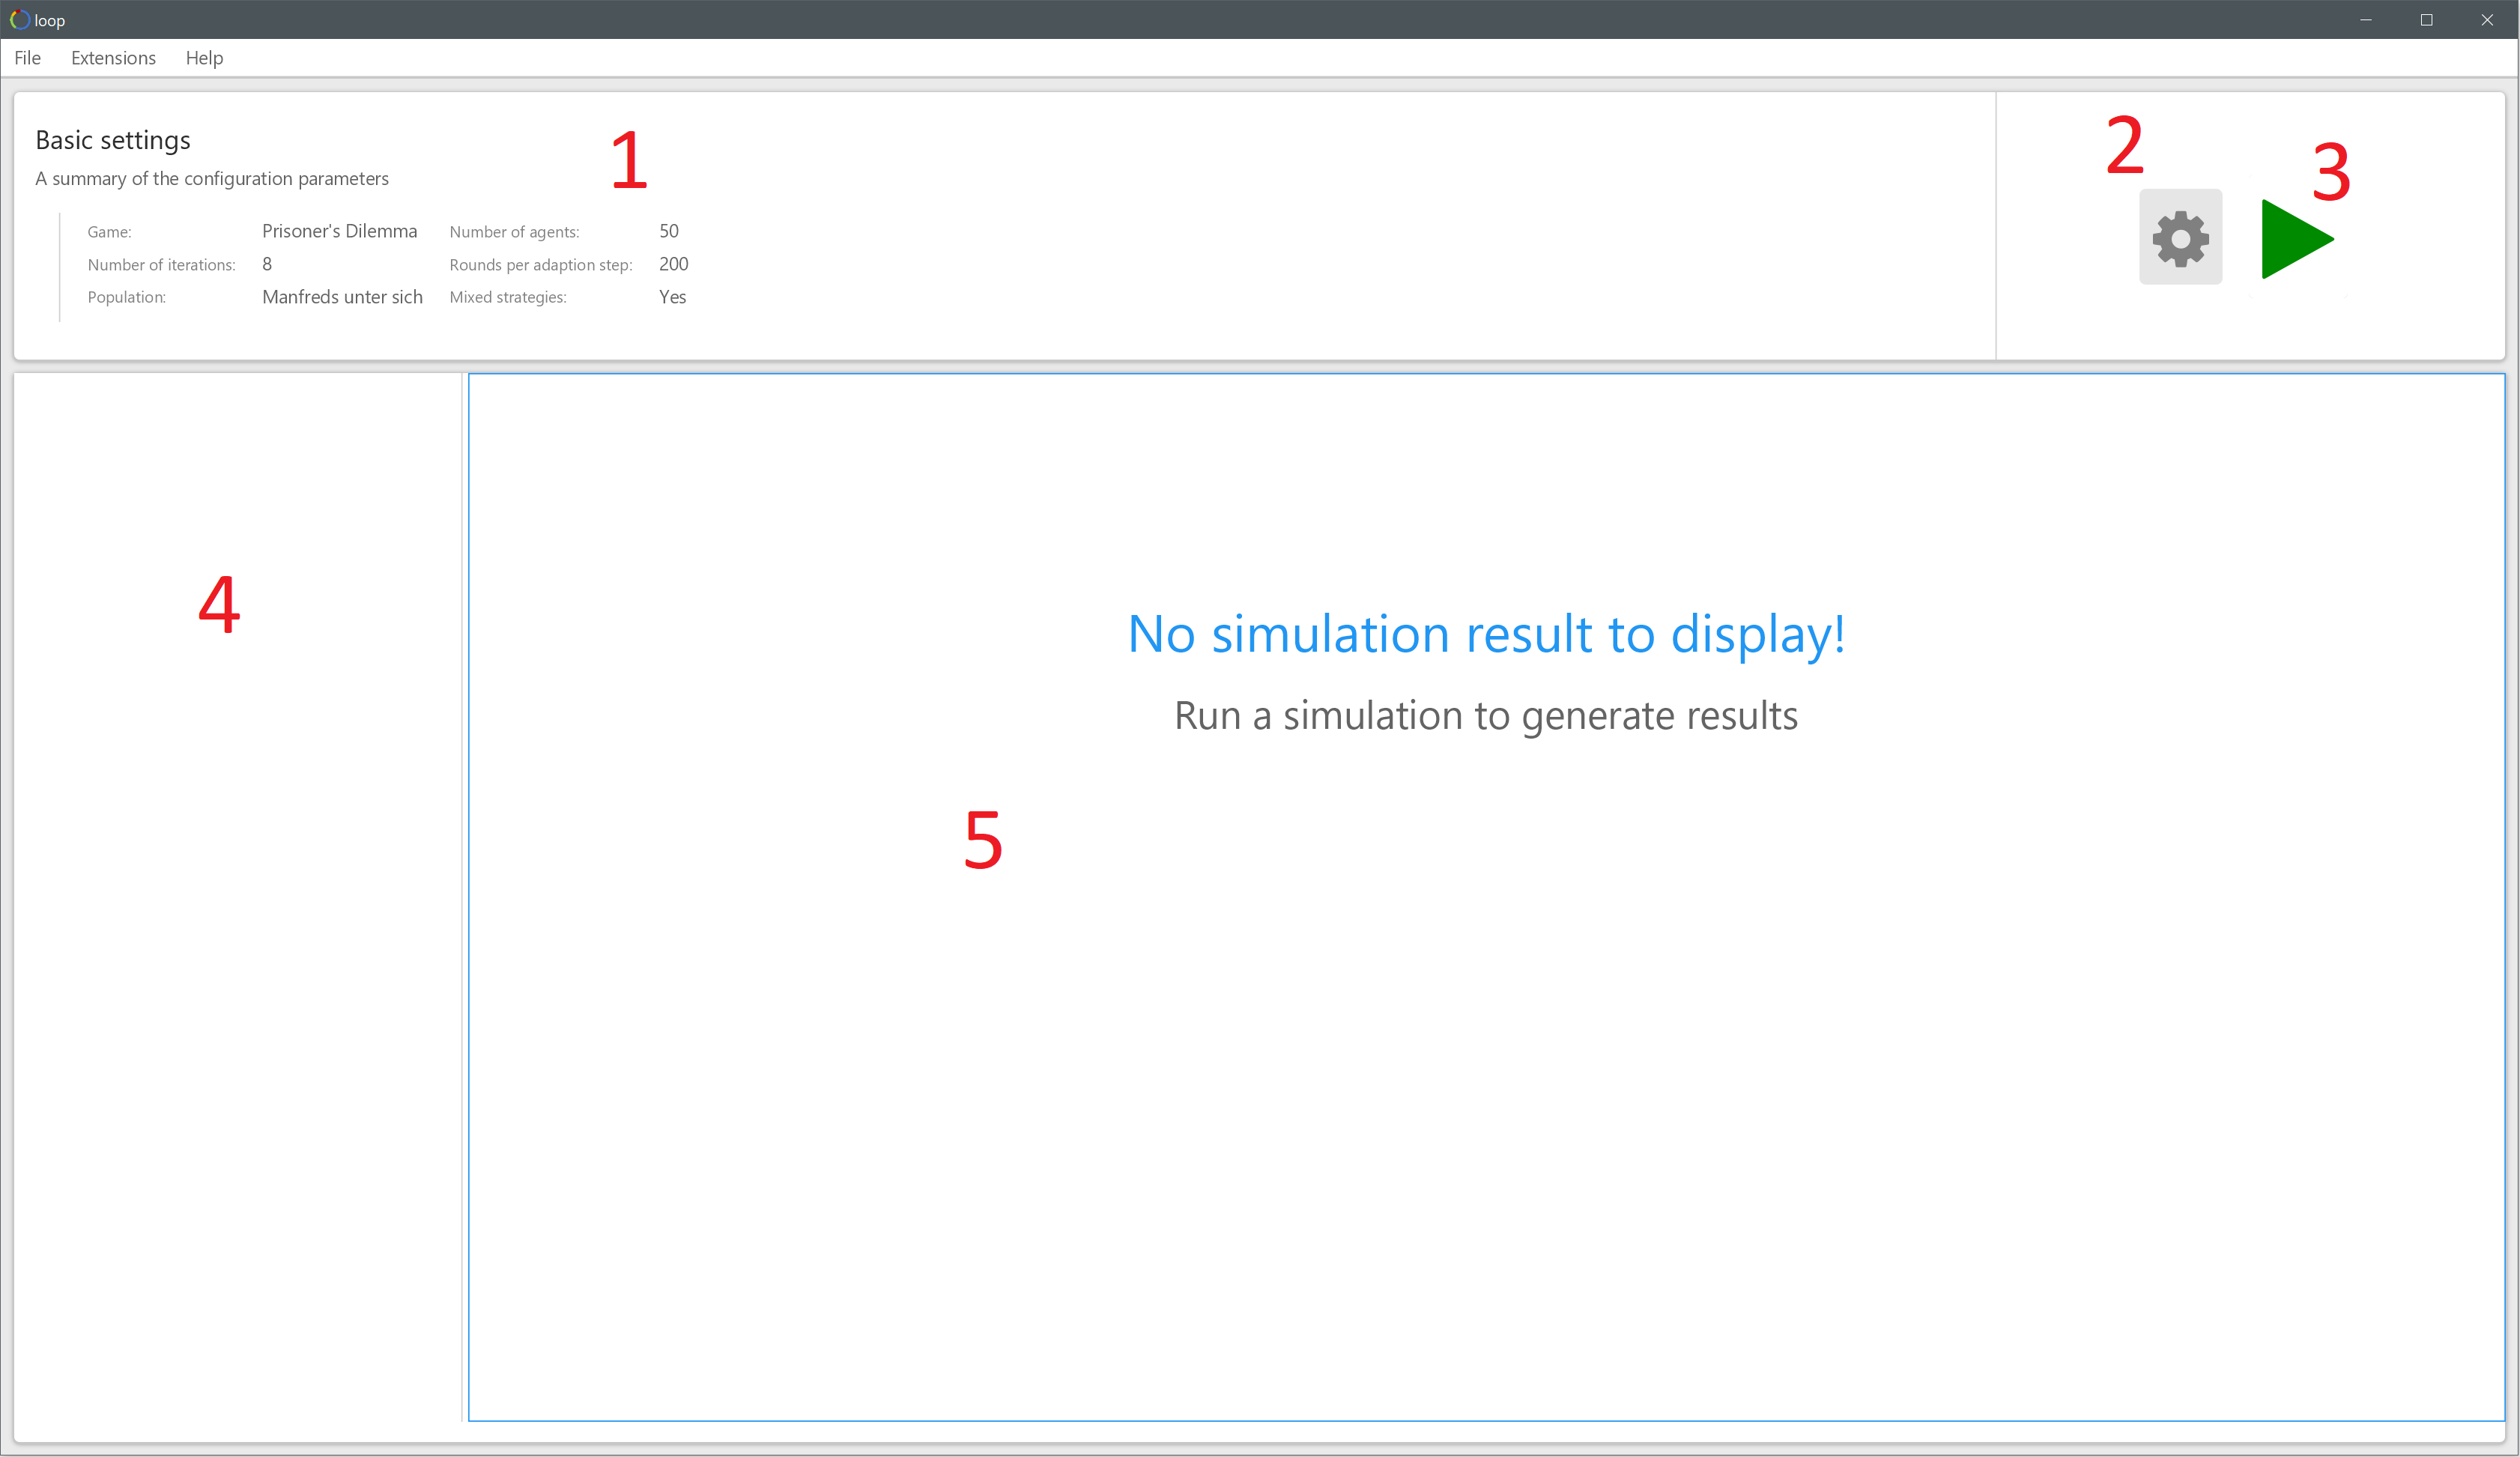
\includegraphics[width=\linewidth]{img_manual/program_start.png}
	\caption{The home window after the first start of the program.}
	\label{fig:program_start}
\end{figure}

\subsection{Edit the configuration}\label{sec:edit_config}
To edit the active configuration, press the cog-labeled button in the home window. This will open up the configuration window (see Fig.\ref{fig:config_window}). On the left-hand side, all configurable parameters of a simulation can be modified. If the selected pairing algorithm, success quantification, strategy adaption mechanism or equilibrium criterion has configurable parameters, they can be entered below the corresponding dropdown menu (see \circled{1} in Fig.\ref{fig:config_window}). On the right-hand side, a short description and a table containing the payoffs of the selected game are displayed (see \circled{2} in Fig.\ref{fig:config_window}). Below (\circled{3} in Fig.\ref{fig:config_window}), a multiconfiguration can be activated, see section \ref{?}.

The  \inlinegraphics{img_manual/rotate_left_button.png} - button will reset all settings to the default configuration. Pressing the  \inlinegraphics{img_manual/check_button.png} - button will close the configuration window and apply the made changes to the active configuration.

\begin{figure}
	\centering
	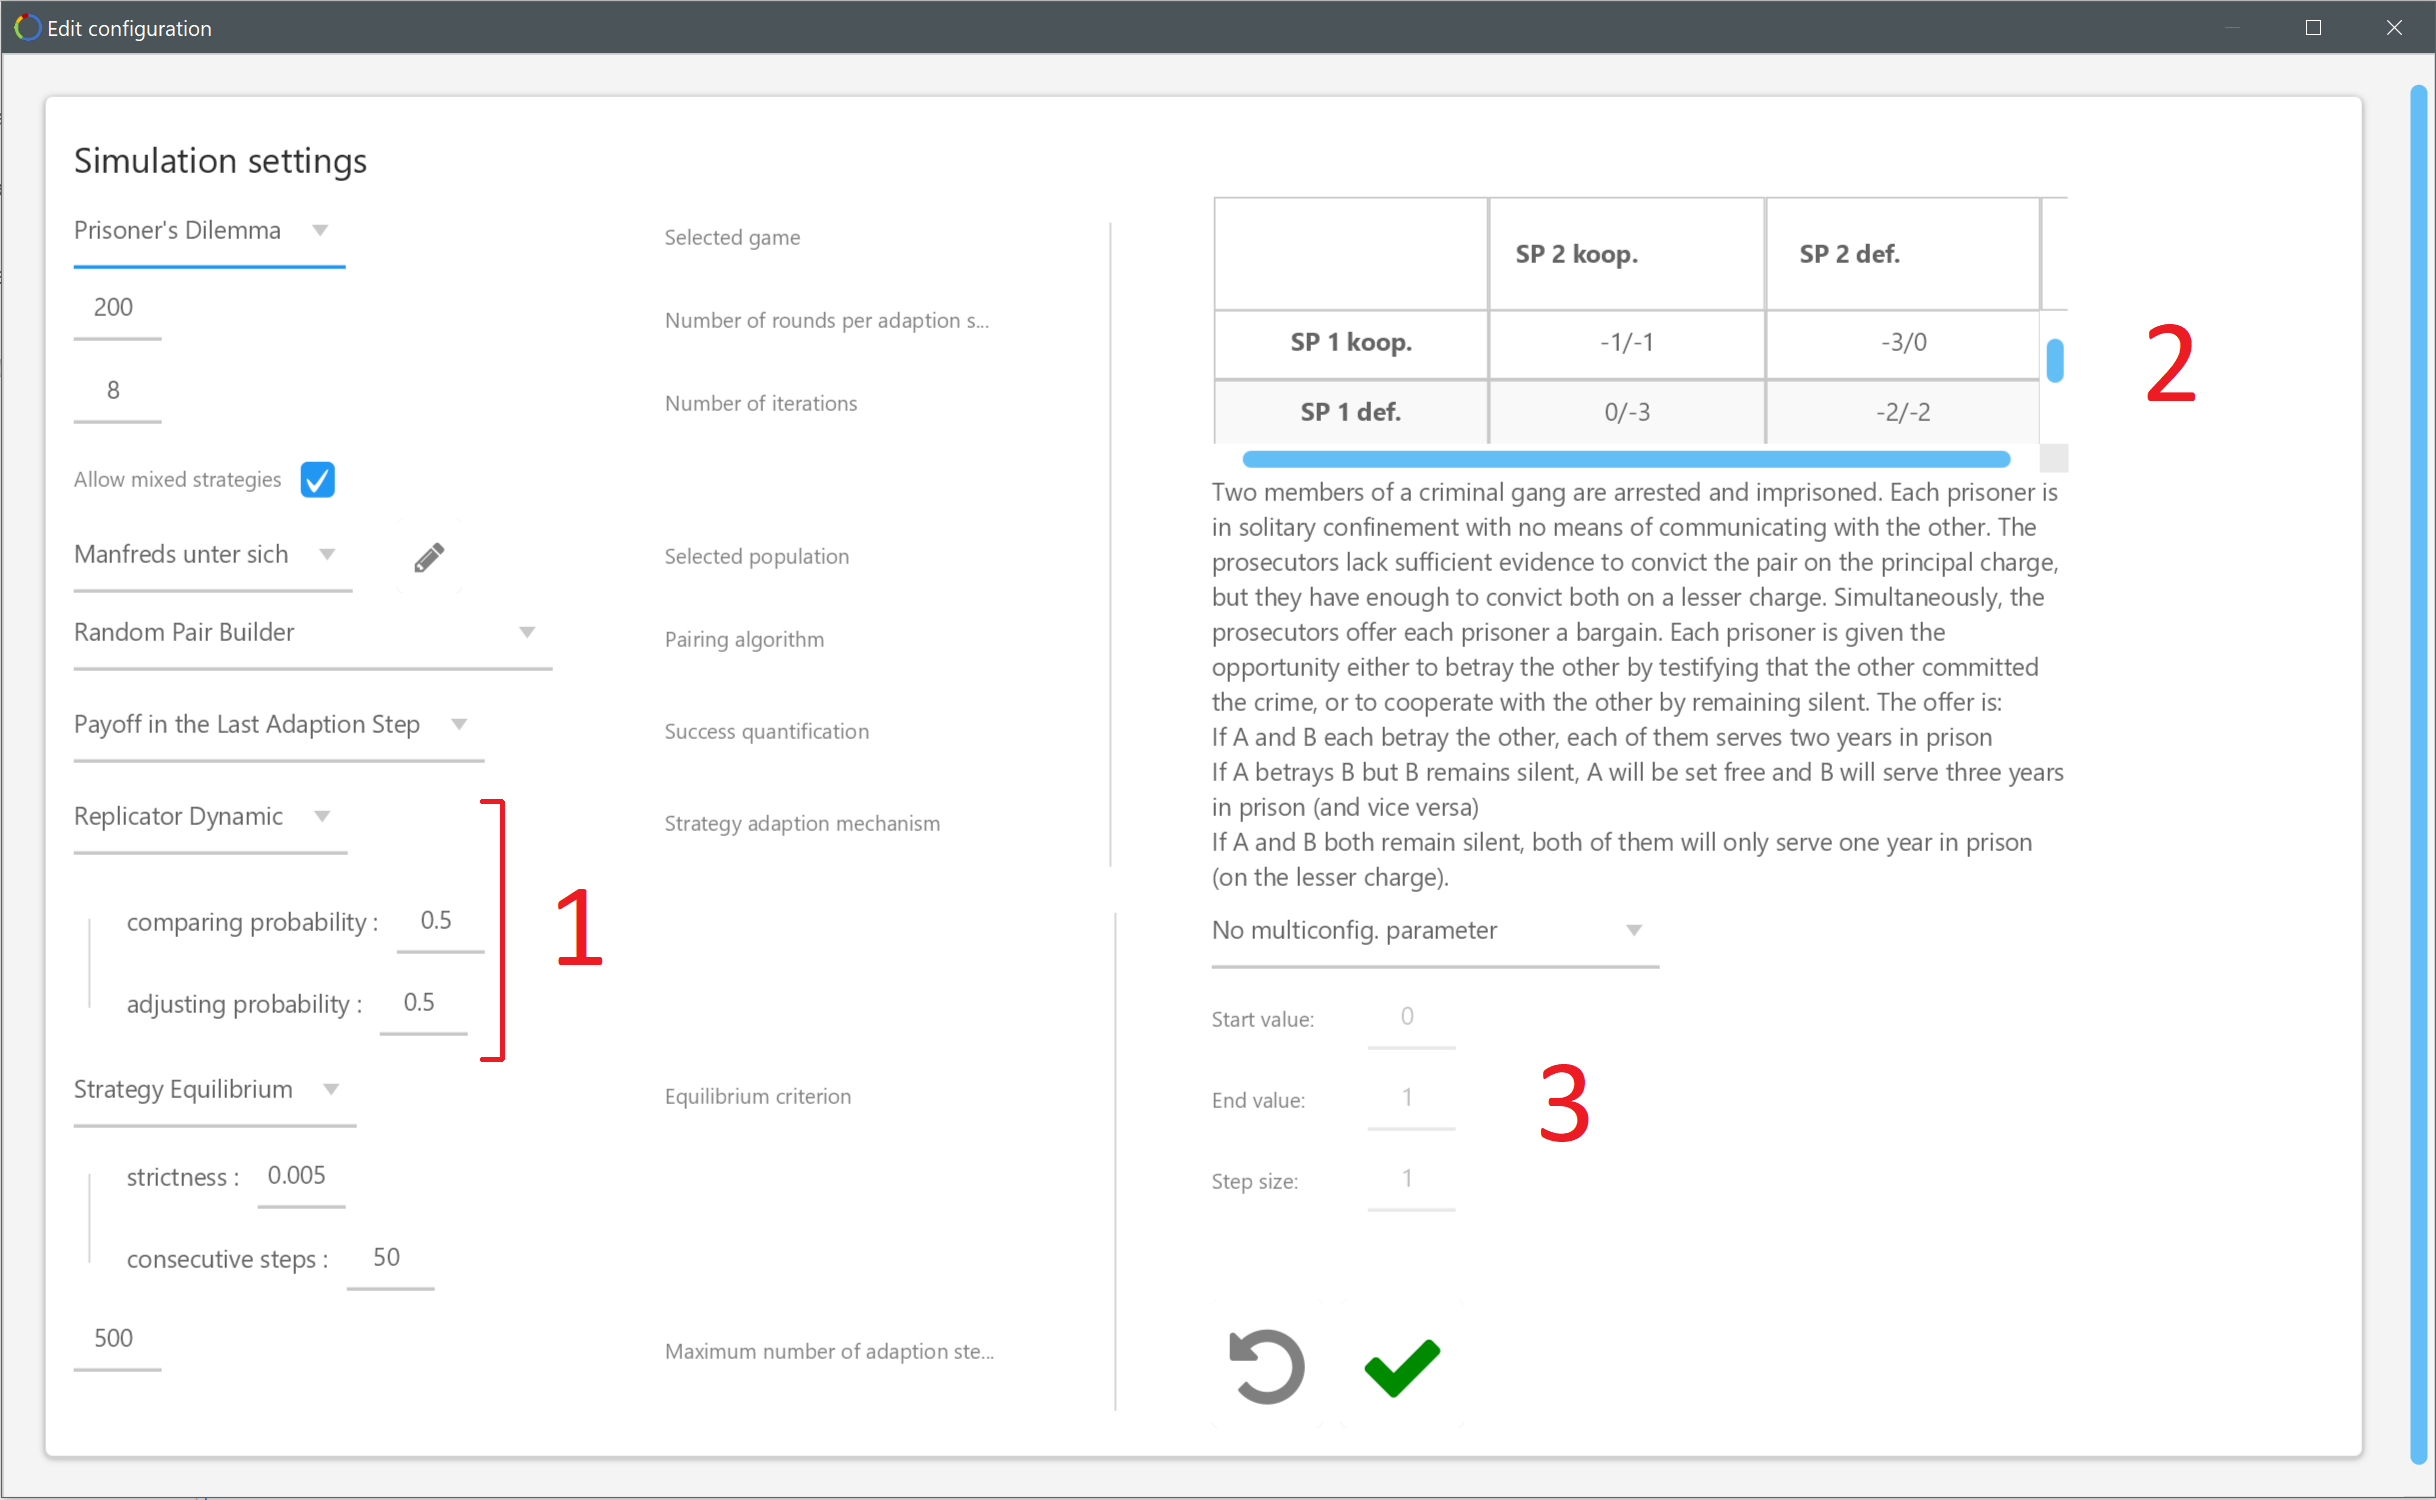
\includegraphics[width=\linewidth]{img_manual/config_window.png}
	\caption{The configuration window.}
	\label{fig:config_window}
\end{figure}

\subsection{Start a simulation}
Pressing the Play-button in the home window will start a simulation with the currently active configuration. It will then appear in the list in the left-hand side area of the home window. The list entry displays an estimate of the time left until the simulation finishes as well as how many iterations have already been executed. If the running simulation is selected, the output view will contain the same information as the list entry as well as a button labeled with an  \inlinegraphics{img_manual/x_button.png}. If pressed, the simulation is cancelled.

\begin{figure}
	\centering
	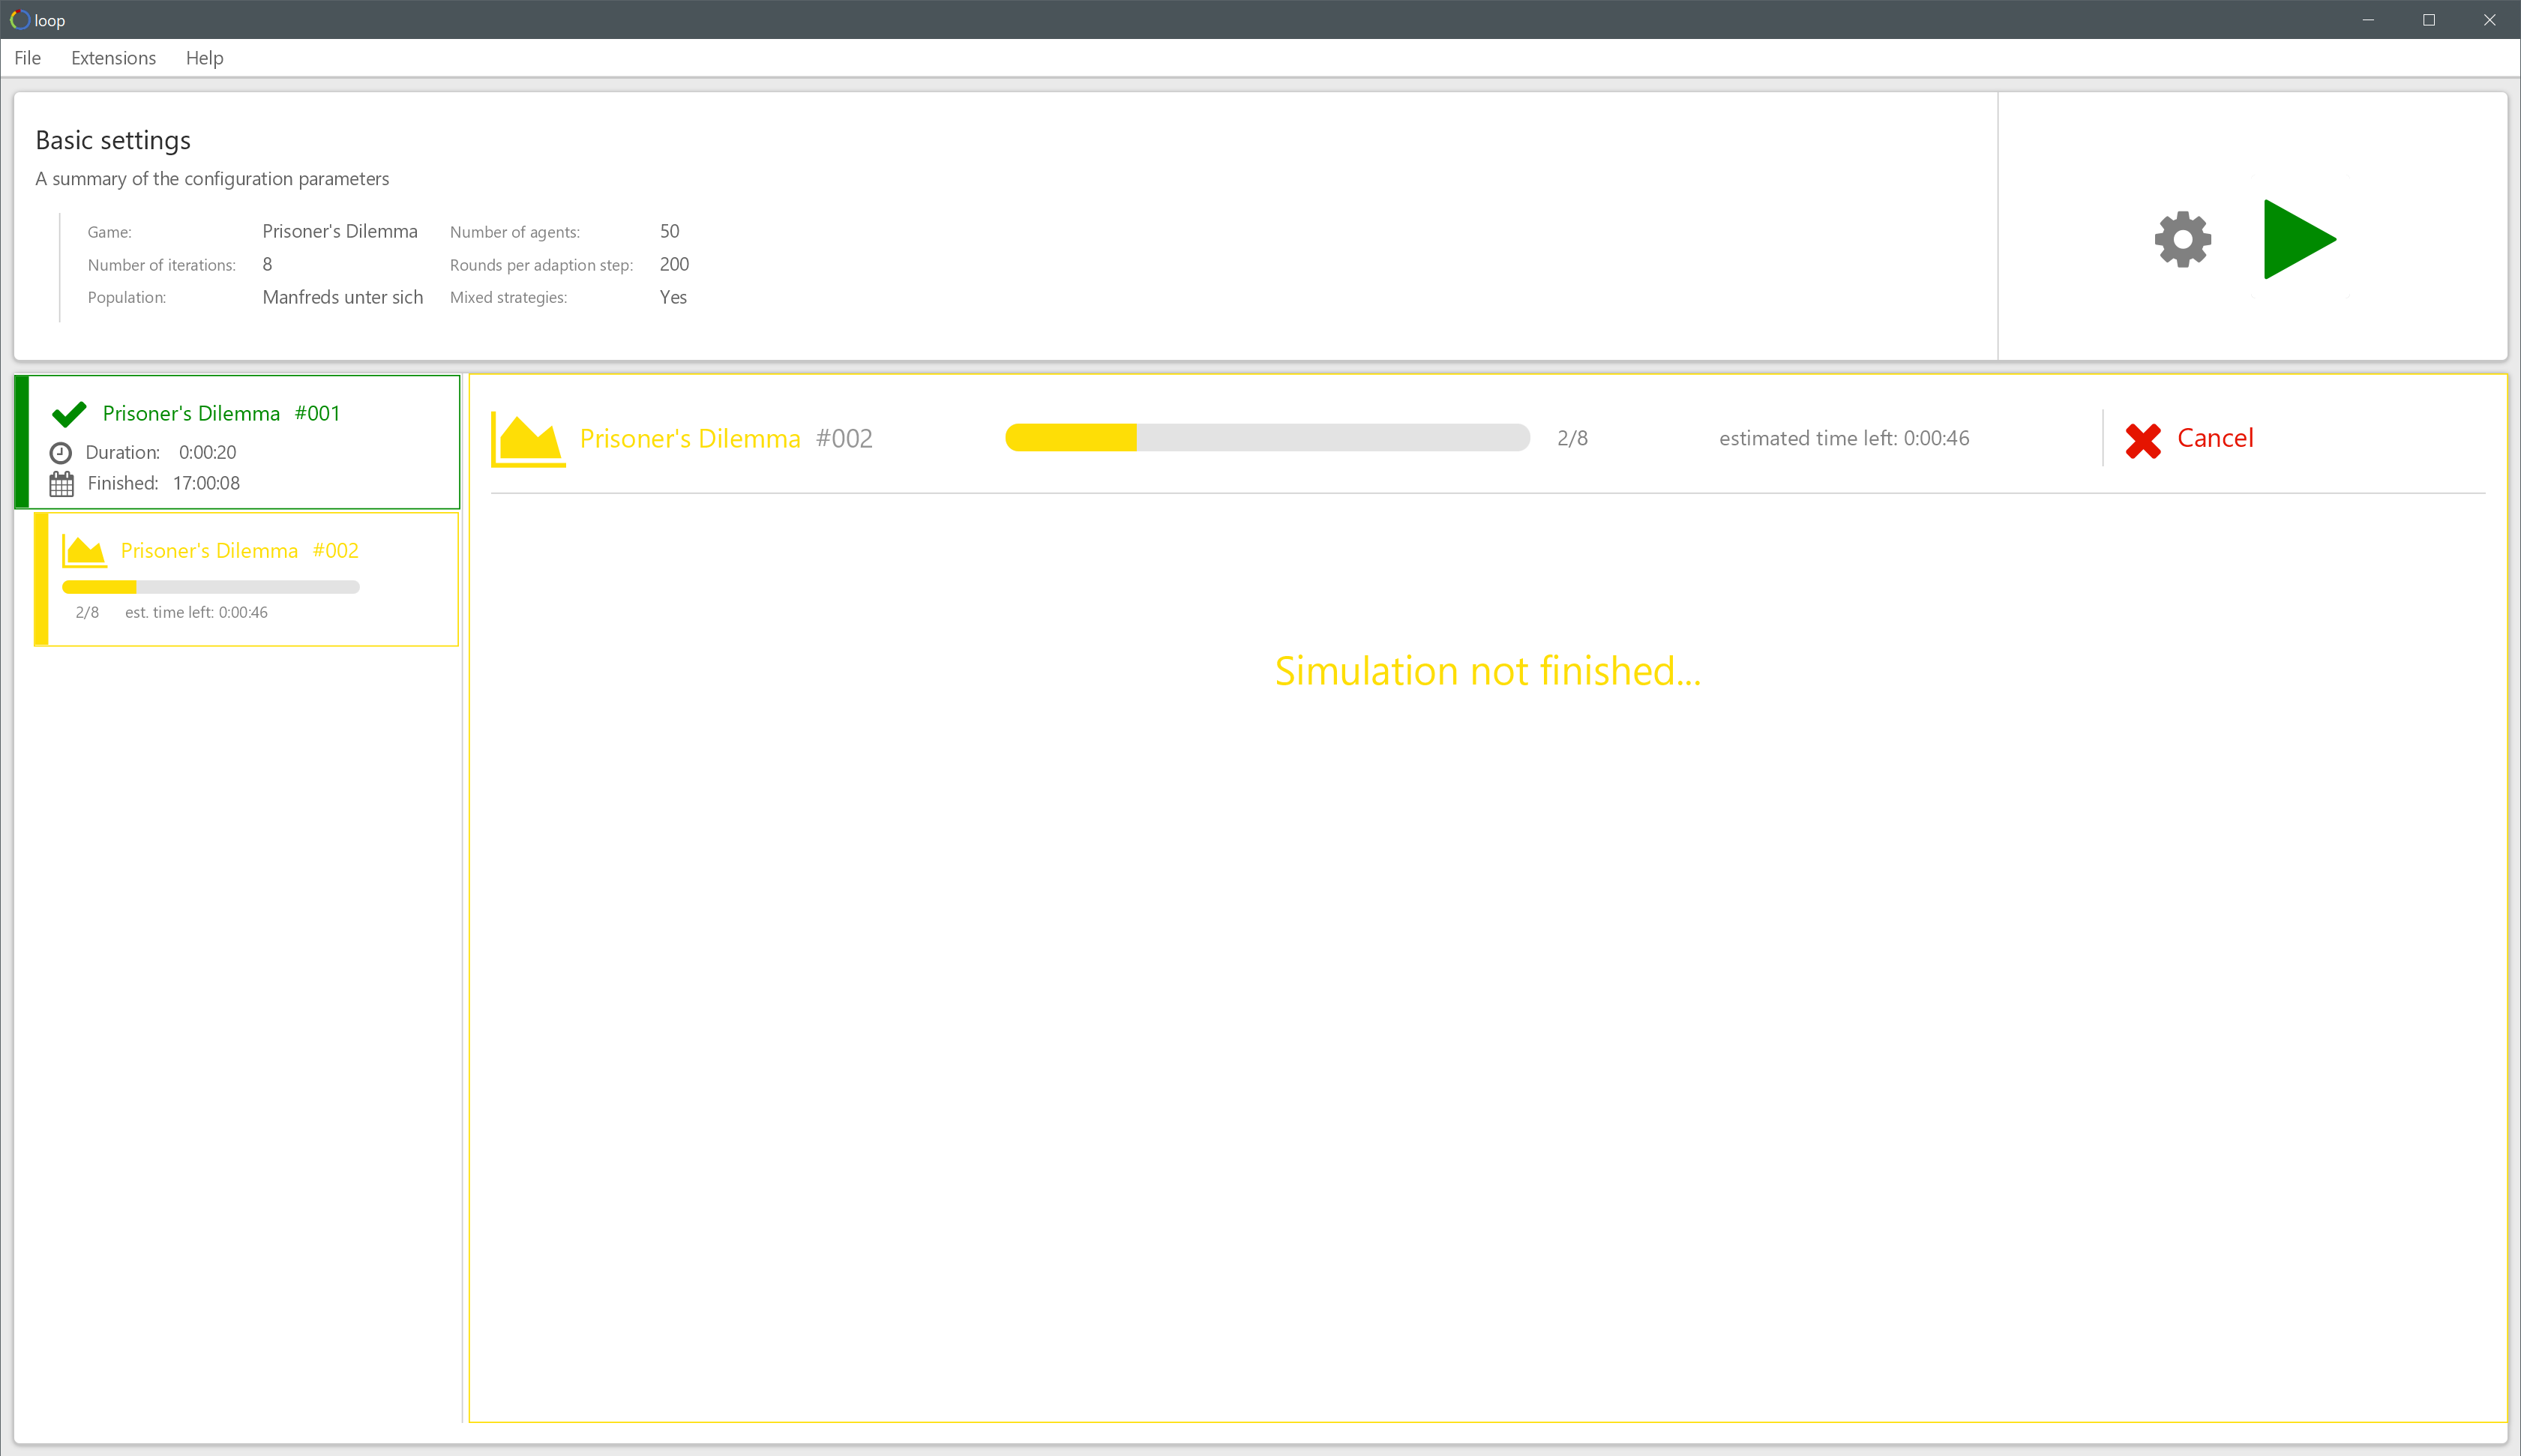
\includegraphics[width=\linewidth]{img_manual/running_simulation.png}
	\caption{The home window with a running simulation selected.}
	\label{fig:running_simulation}
\end{figure}

\subsection{View the simulation results}
As soon as a simulation is finished, its list entry turns green and displays time and date of the moment it finsihed as well as the duration of its execution:
\begin{figure}[h]
	\centering
	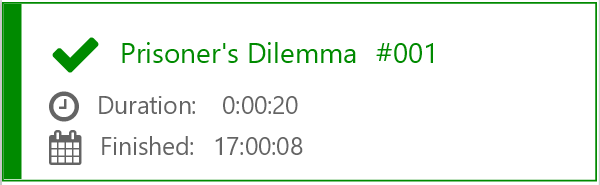
\includegraphics[width=0.3\linewidth]{img_manual/finished_simulation_list_entry.png}
\end{figure}\\
If selected, the output view will display detailed information about the simulations results. The output is divided into two subpages: the \enquote{Detailed output} and the \enquote{Abstracted output}. To switch between the two, the  \inlinegraphics{img_manual/arrow_left_button.png} and  \inlinegraphics{img_manual/arrow_right_button.png} buttons at the bottom of the output view can be used.

\subsubsection{Detailed Output}
\begin{figure}
	\centering
	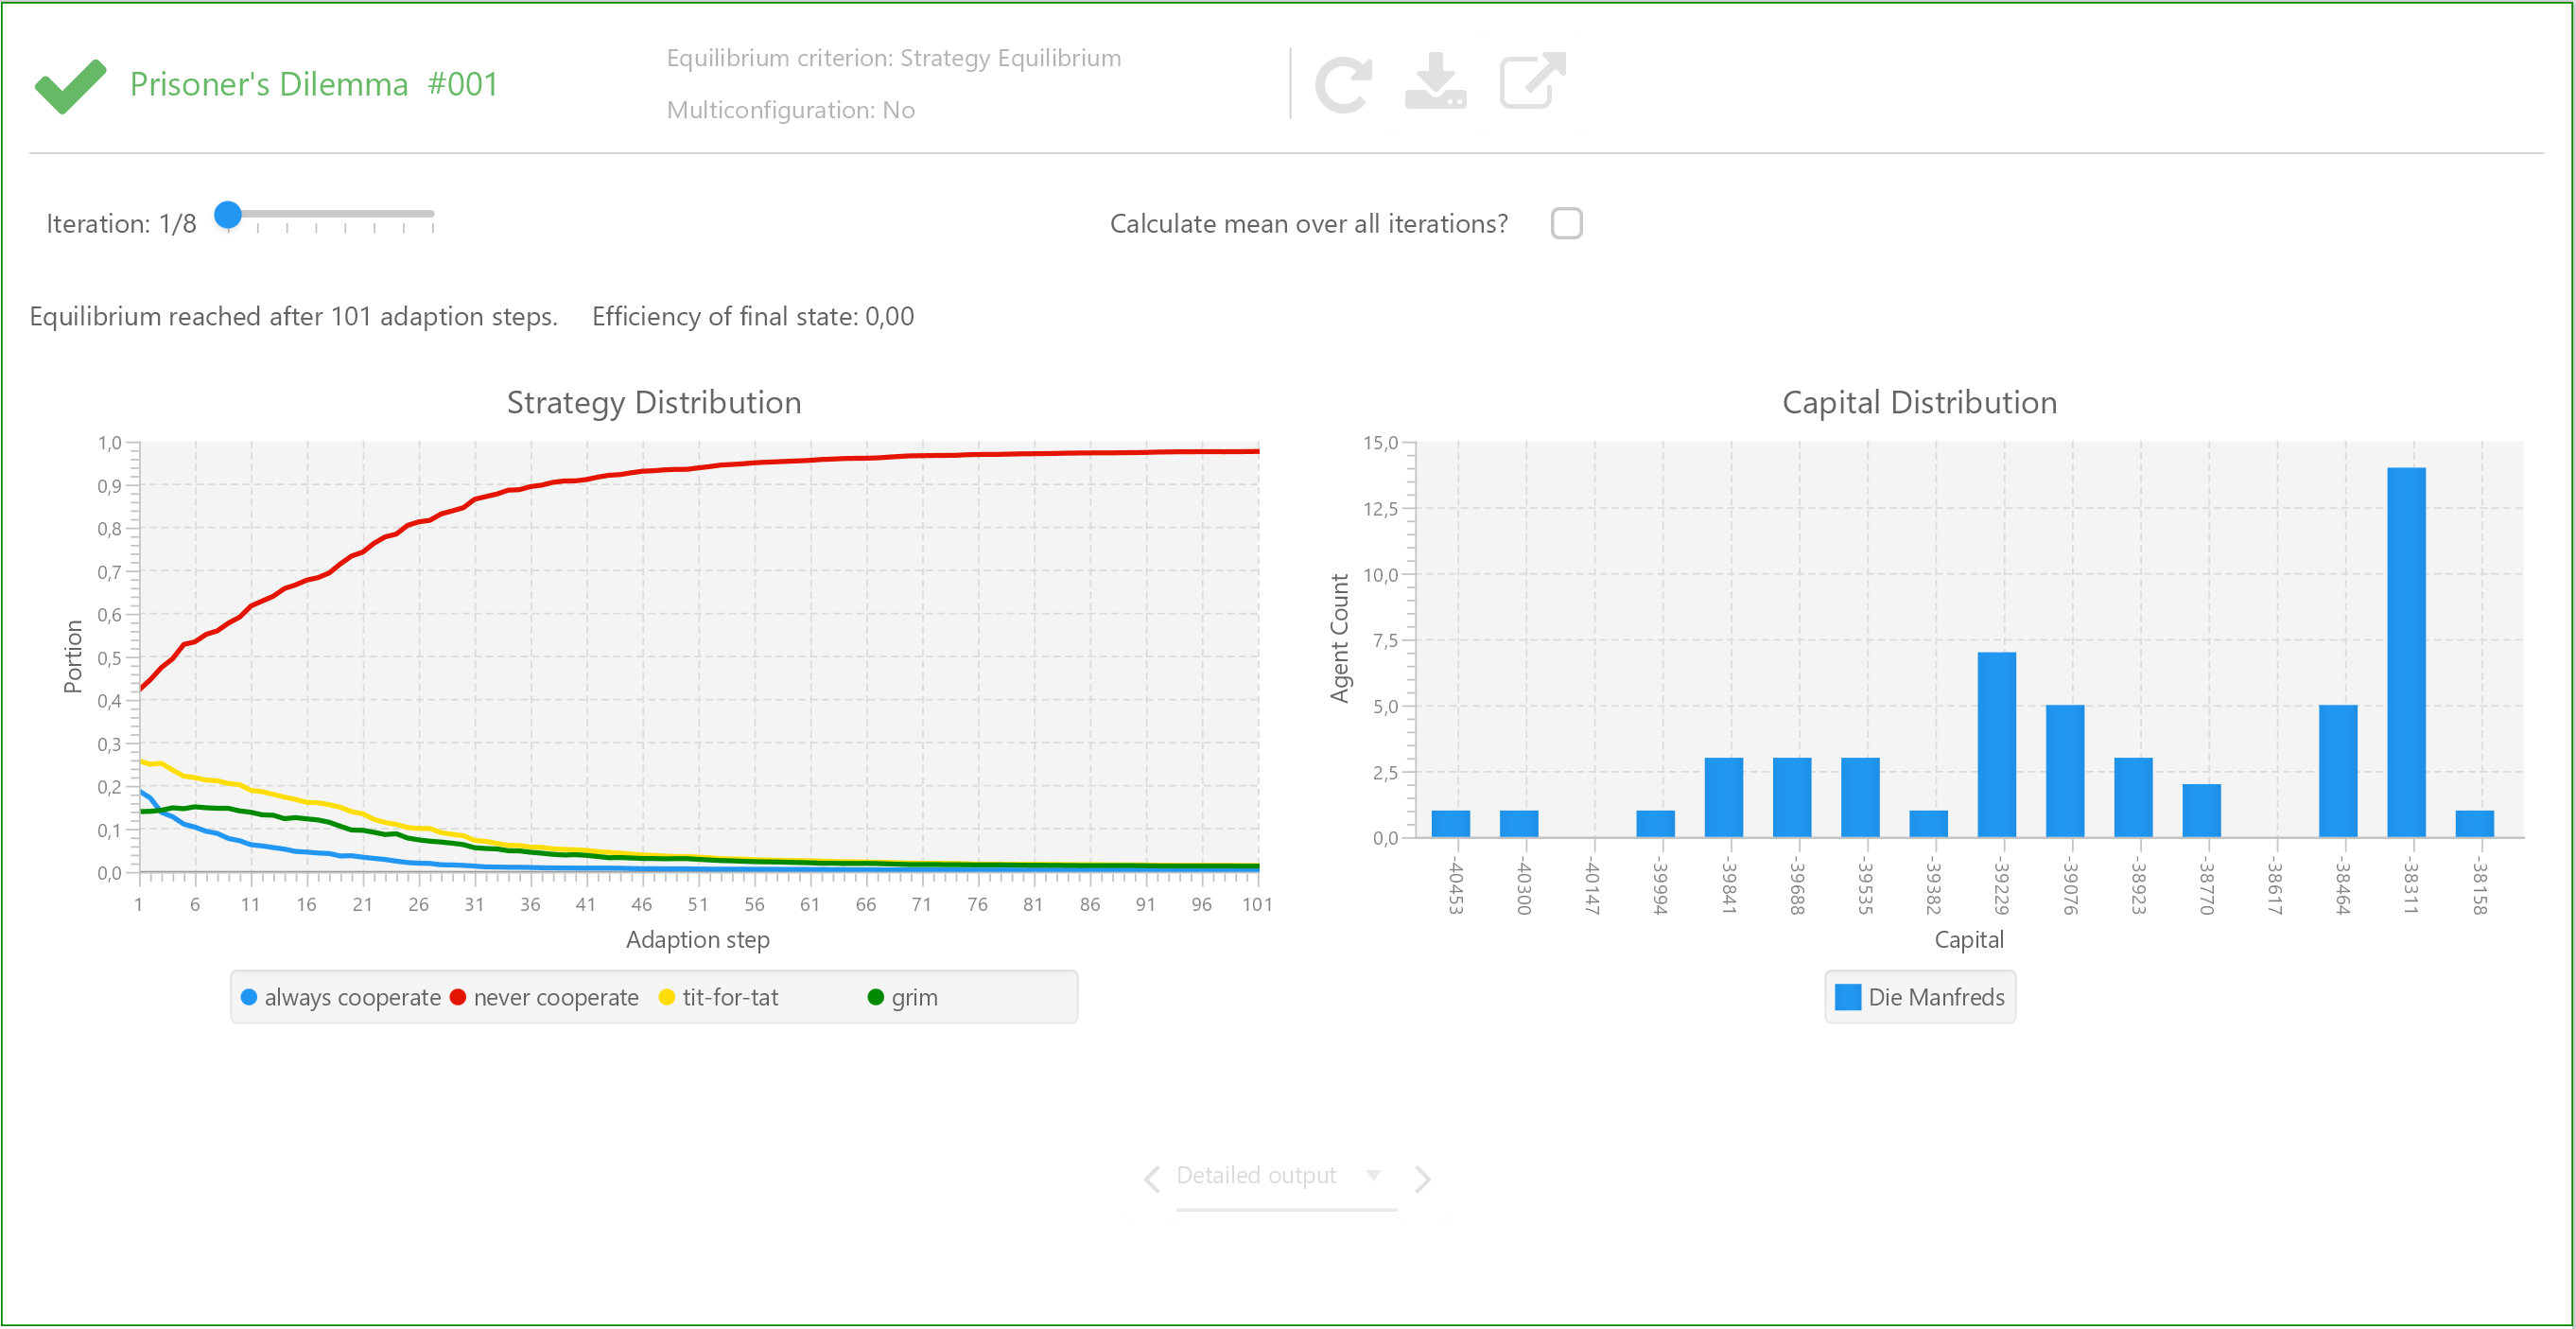
\includegraphics[width=\linewidth]{img_manual/detailed_output.png}
	\caption{The detailed output.}
	\label{fig:detailed_output}
\end{figure}
In the detailed output (see Fig.\ref{fig:detailed_output}), information about strategy and capital distribution of the agents are displayed for any selected iteration. To select an iteration, use the correspondingly labeled slider at the top of the output view \circled{1}. The iterations are sorted by their final efficiency, i.e. in the case of Fig.\ref{fig:detailed_output}, iteration \(1/8\) is the least, iteration \(8/8\) the most efficient among the eight executed iterations.

\textbf{Strategy distribution:} The line chart labeled \enquote{Strategy distribution} \circled{2} displays the evolution of the mixture of strategies used by the agents over the time of the simulation. It contains one line for every used (pure) strategy. Each line indicates the relative frequency of the corresponding strategy being used by agents in every single adaption step. For example, consider the strategy distribution displayed in Fig.\ref{fig:strategy_distribution}. It tells us that in the beginning of the simulation, all strategies appeared with a similar frequency of \(21\%\) to \(29\%\). Towards the end, \enquote{grim} prevailed with a frequency of about \(70\%\), while \enquote{never cooperate} and \enquote{tit for tat} dropped below \(20\%\) and \enquote{always cooperate} basically vanished.

\begin{figure}[h]
	\centering
	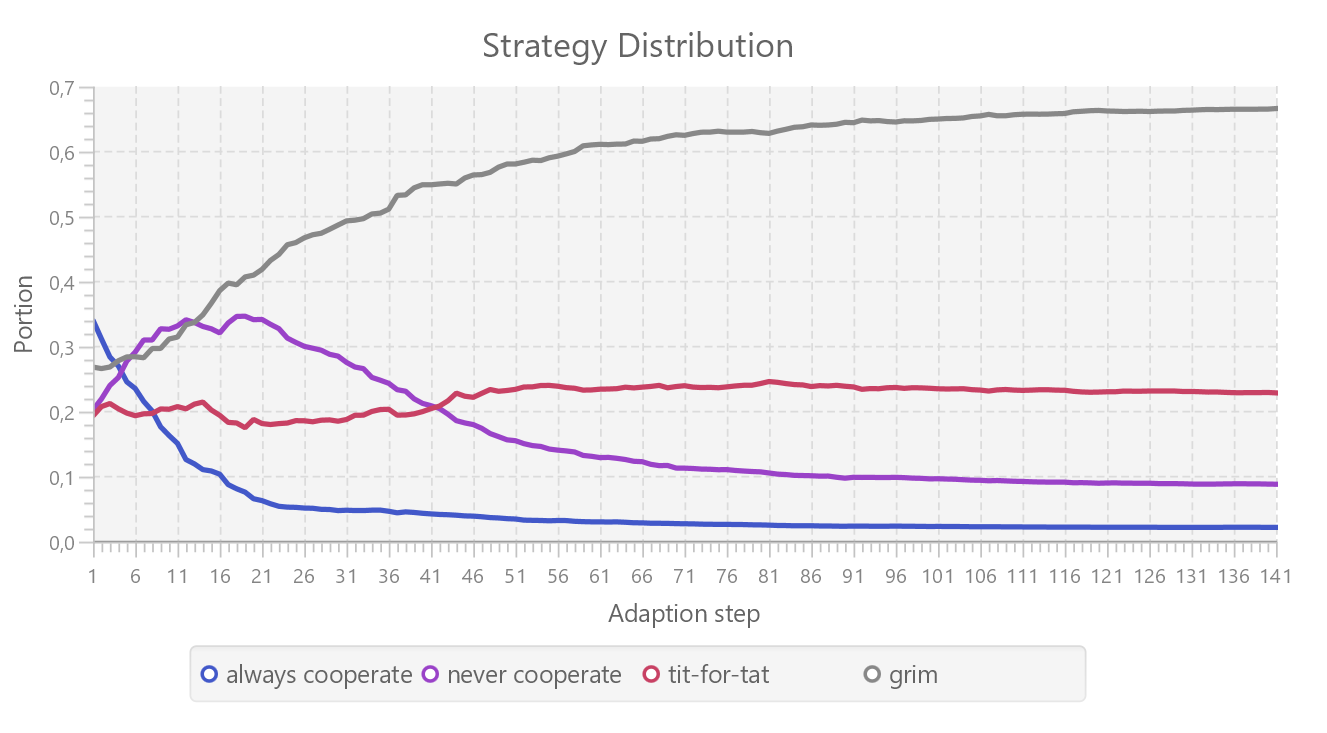
\includegraphics[width=0.8\linewidth]{img_manual/strategy_distribution.png}
	\caption{An exemplary strategy distribution.}
	\label{fig:strategy_distribution}
\end{figure}

\textbf{Capital distribution:} The bar chart labeled \enquote{Capital distribution} \circled{3} displays a histogramm of the final total capitals of all agents at the end of the simulation. The width of the bins of the histogram are chosen in a way such that there is always about \(15\) bins. Each bin is then labeled with the mean of the interval covered by it. Note that final capitals might be negative (as in Fig.\ref{fig:capital_distribution}) if the payoffs of the used game are negative (such as in the prisoner's dilemma).

\begin{figure}[h]
	\centering
	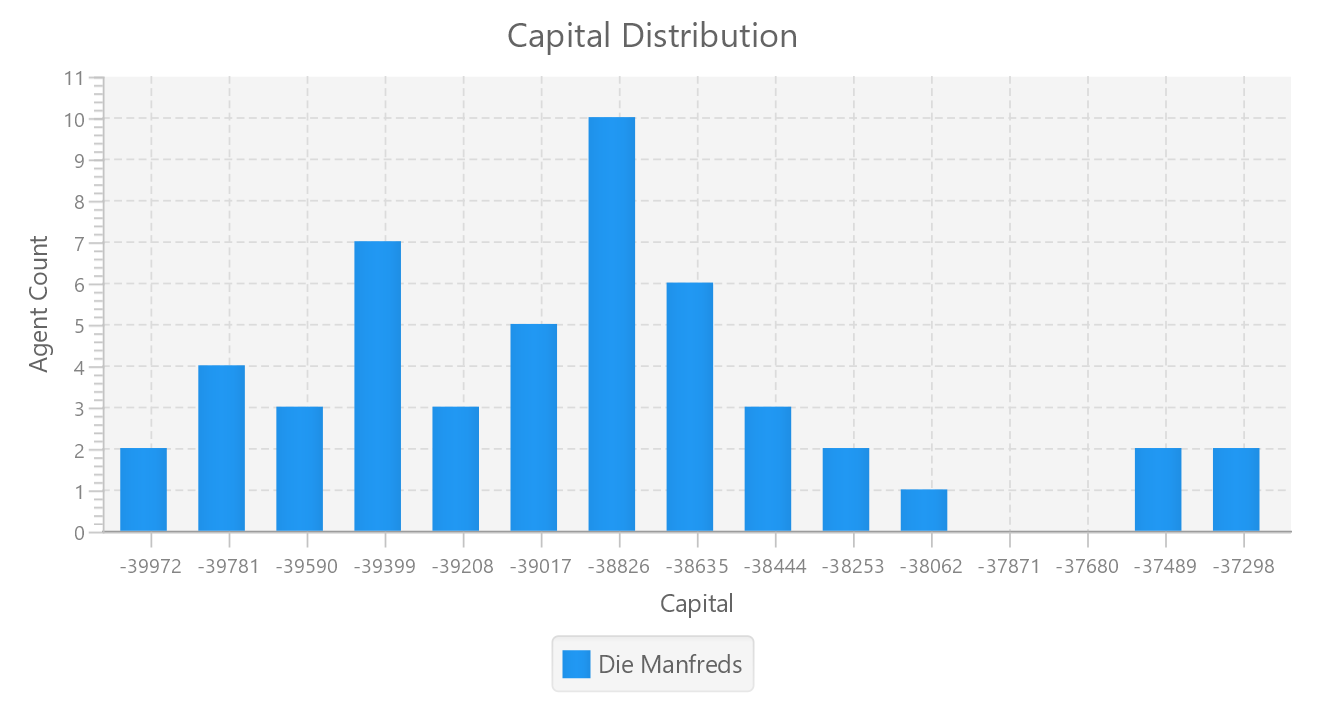
\includegraphics[width=0.8\linewidth]{img_manual/capital_distribution.png}
	\caption{An exemplary capital distribution.}
	\label{fig:capital_distribution}
\end{figure}

\subsubsection{Abstracted Output}
\begin{figure}
	\centering
	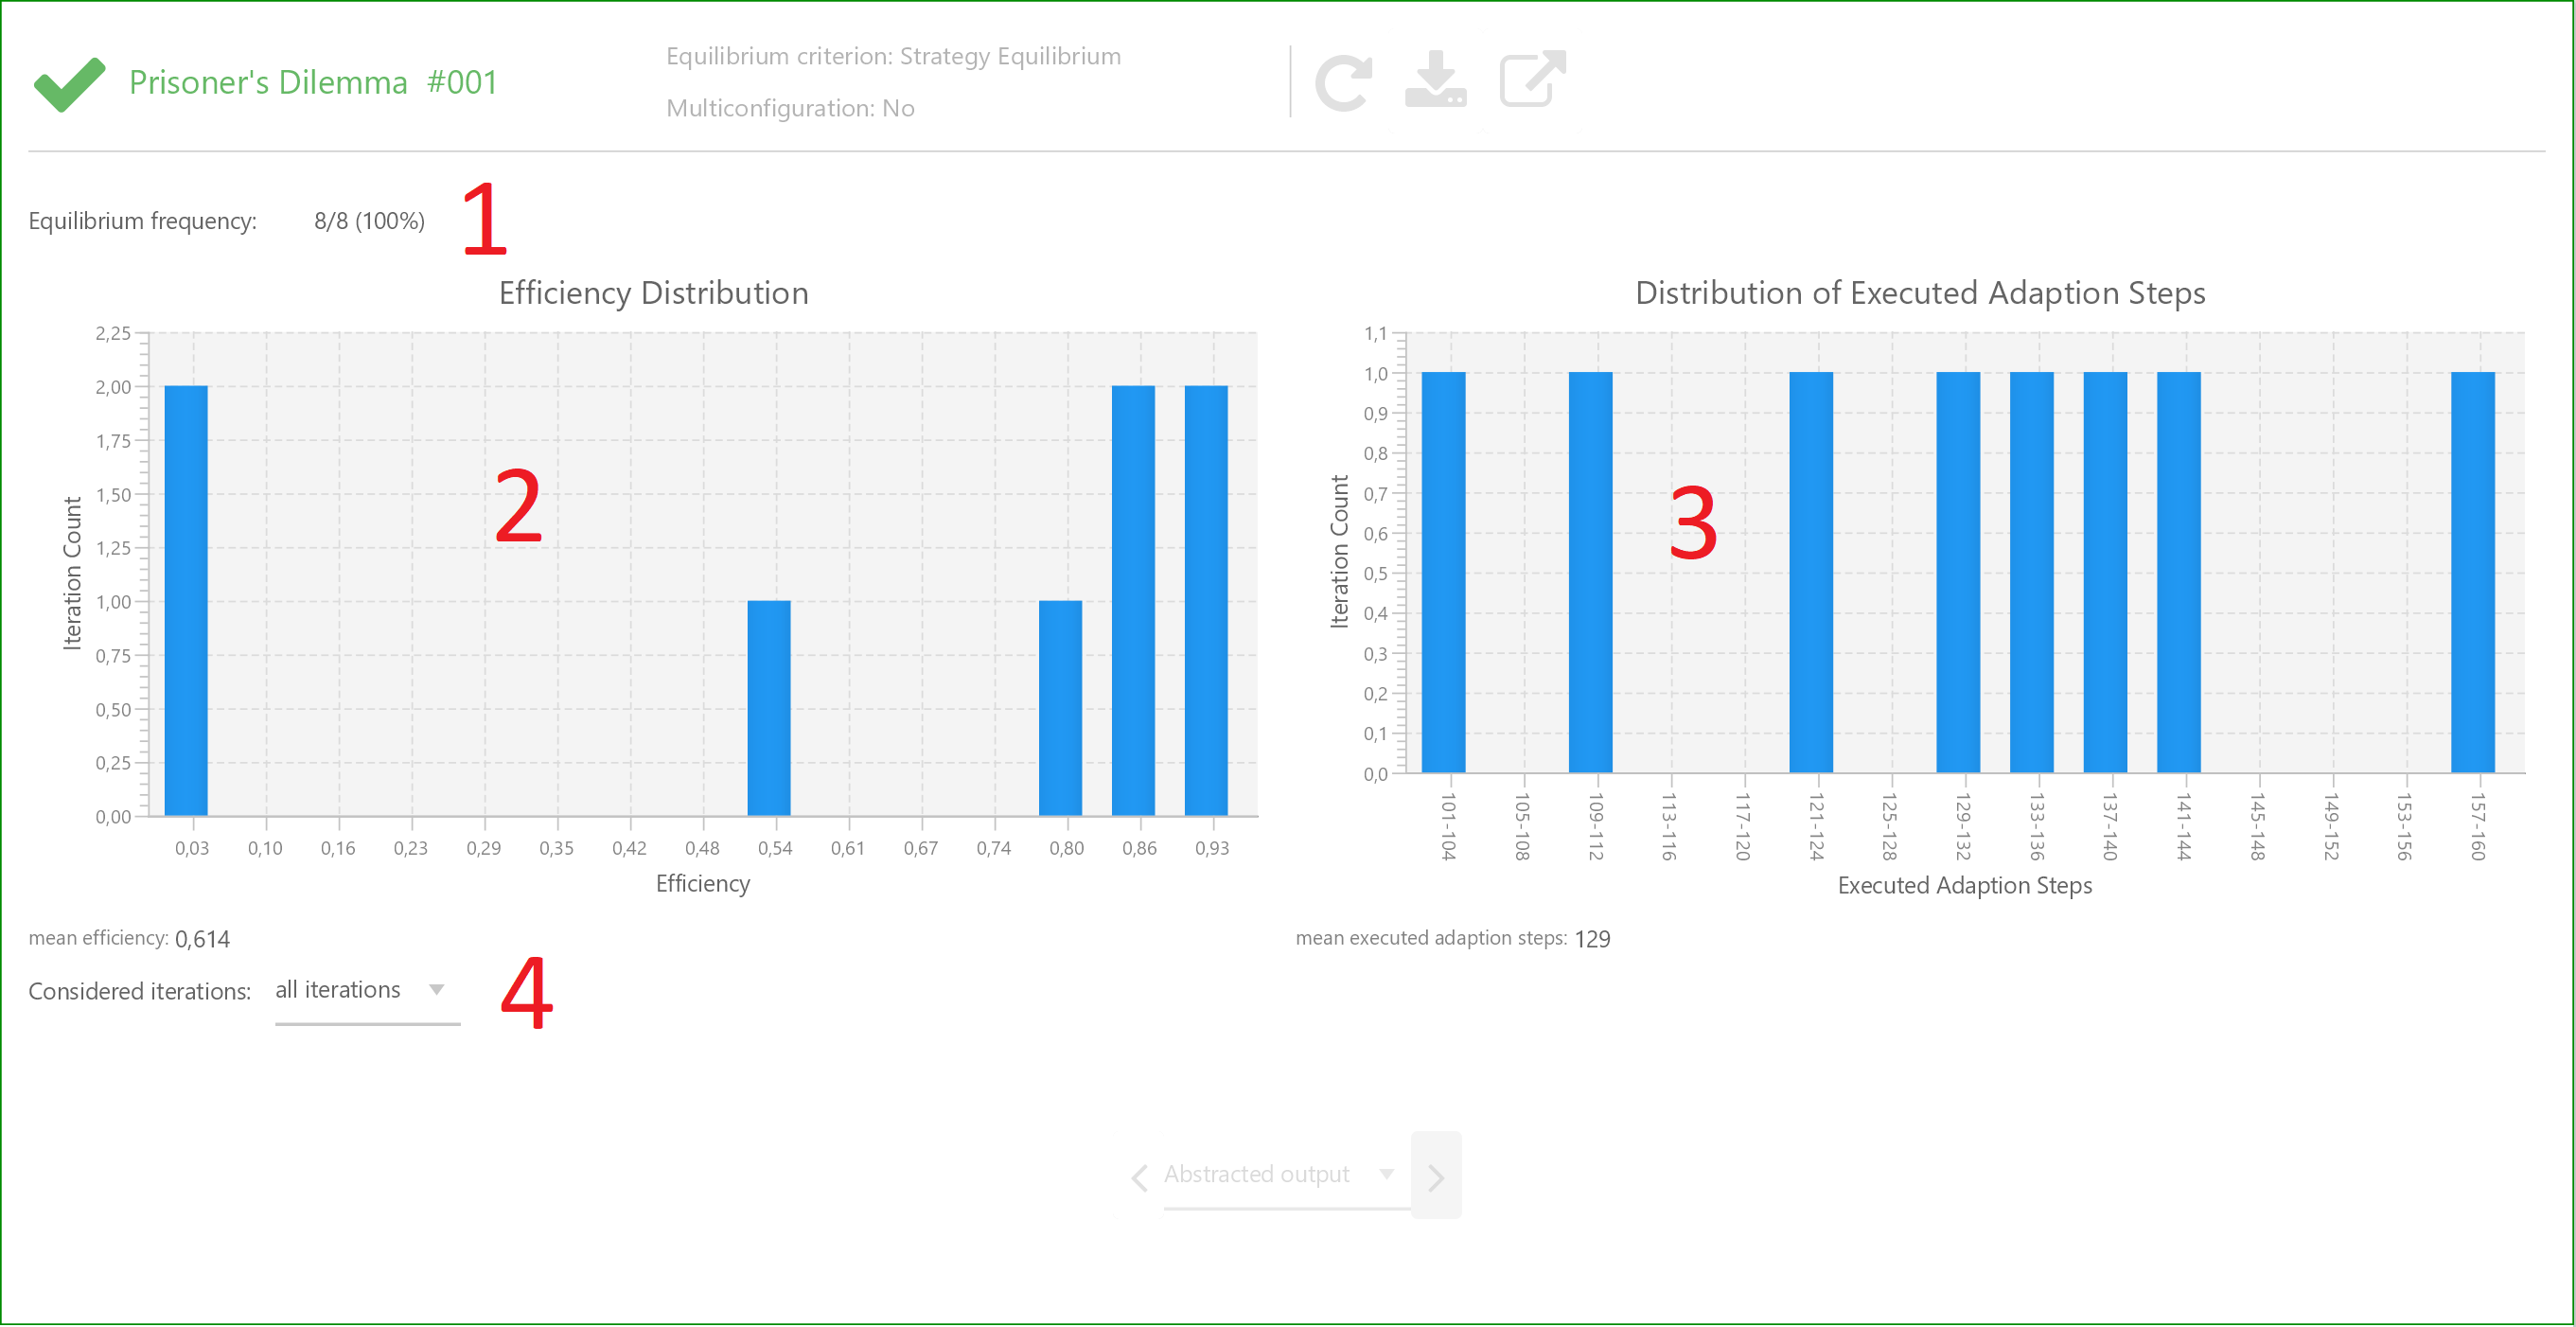
\includegraphics[width=\linewidth]{img_manual/abstracted_output.png}
	\caption{The abstracted output.}
	\label{fig:abstracted_output}
\end{figure}
The abstracted output (see Fig.\ref{fig:abstracted_output}) contains information abstracted from all executed iterations. At the top \circled{1} the \enquote{equilibrium frequency}, i.e. the portion of all iterations in which an equilibrium was reached is displayed. Below reside two histograms, the \enquote{Efficiency distribution} and the \enquote{Distribution of executed adaption steps}.

\textbf{Efficiency distribution}: The efficiency distribution \circled{2} is a histogram of the final efficiencies of all executed iterations. Consider Fig.\ref{fig:efficiency_distribution}. In the corresponding simulation, five iterations finished with an efficiency of around \(0.9\) and the other three with efficiencies \(0.67\), \(0.42\) and \(0.04\) respectively. Again, bin width is chosen such that there is around \(15\) bins in total and the labels display the mean of the interval covered by the bins. Below the strategy distribution, the mean efficiency of all iterations is displayed, in this case \(0.722\) (see Fig.\ref{fig:abstracted_output}).

\begin{figure}[h]
	\centering
	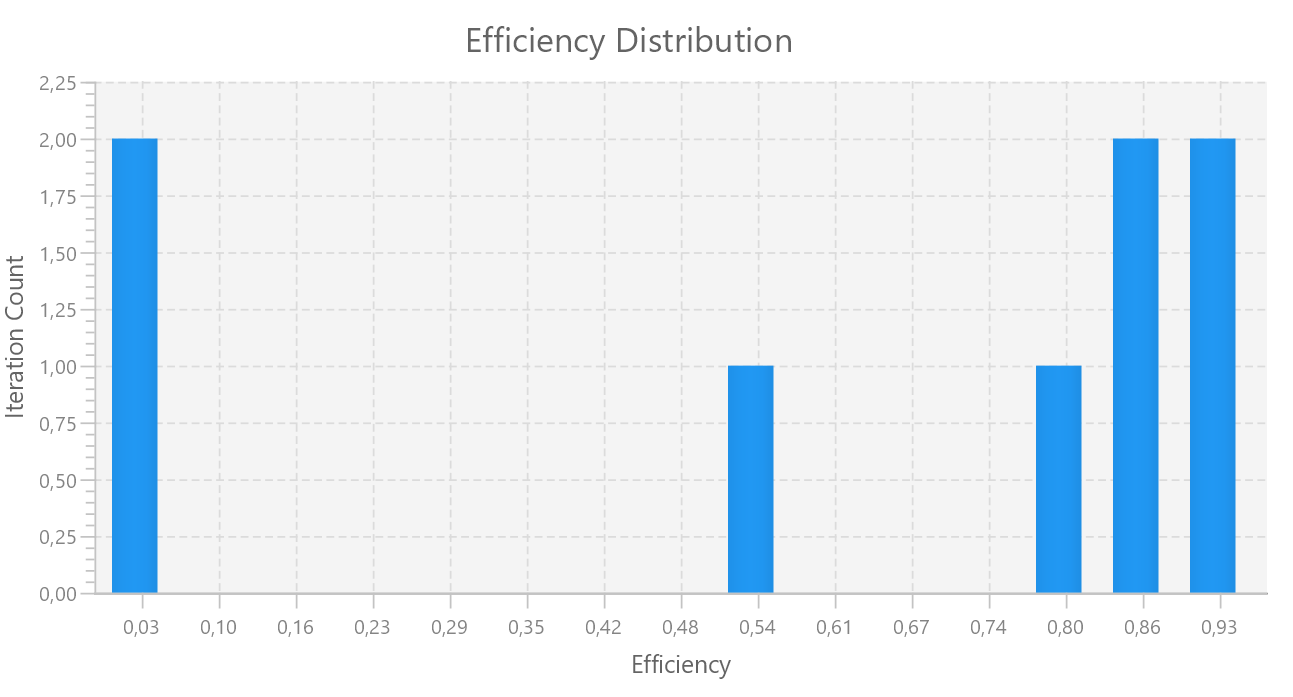
\includegraphics[width=0.8\linewidth]{img_manual/efficiency_distribution.png}
	\caption{An exemplary efficiency distribution.}
	\label{fig:efficiency_distribution}
\end{figure}

\textbf{Distribution of executed adaption steps}: This chart \circled{3} is a histogram of the amount of executed adaption steps of all iterations. Consider Fig.\ref{fig:adapts_distribution}. In the corresponding simulation, all but one iteration finished after \(120\) to \(134\) adaption steps, just one took around \(160\). Below the distribution, the mean amount of executed adaption steps is displayed, in this case \(131\) (see Fig.\ref{fig:abstracted_output}).

\begin{figure}[h]
	\centering
	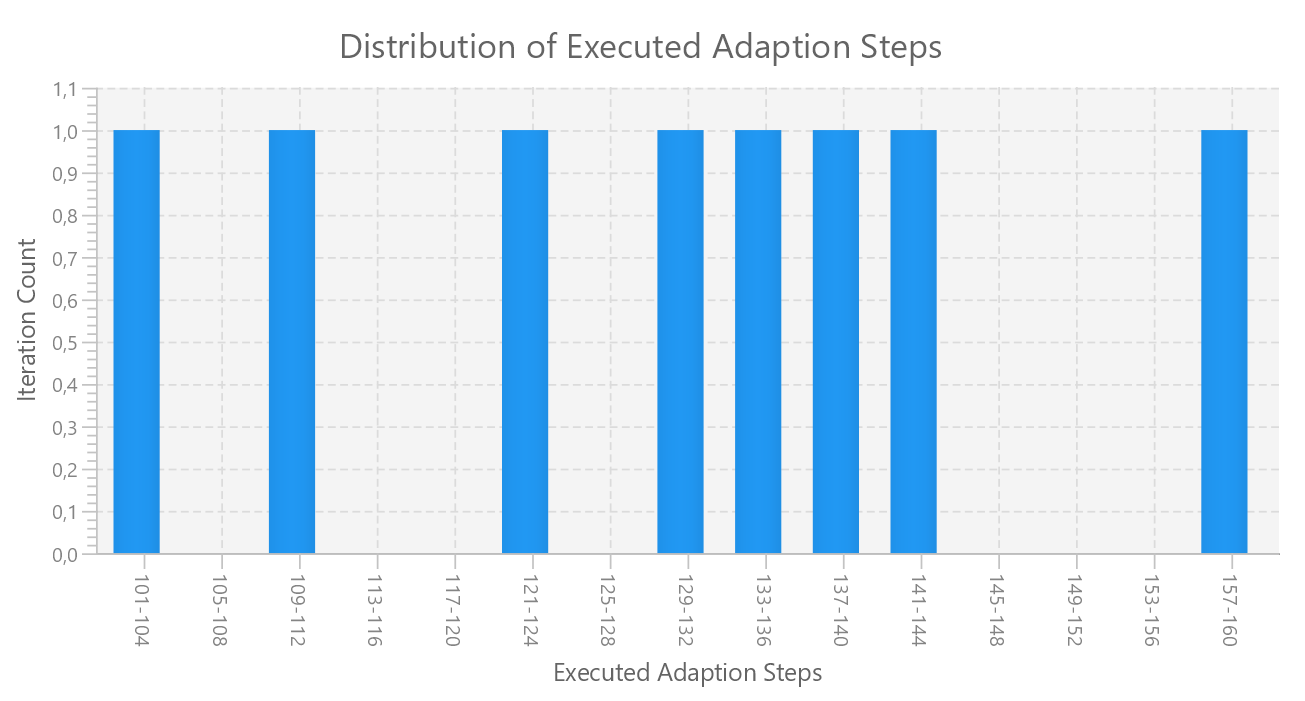
\includegraphics[width=0.8\linewidth]{img_manual/adapts_distribution.png}
	\caption{An exemplary distribution of executed adaption steps.}
	\label{fig:adapts_distribution}
\end{figure}

Below the charts resides a dropdown menu labeled \enquote{Considered iterations} \circled{4}. It can be used to determine whether all iterations or just the ones where an equilibrium (or no equilibrium) was reached shall be included in the calculation of the histograms above.

\subsection{Save the result}
If you whish to save the result of a simulation so you can take a look at it again later, you may do so by clicking the  \inlinegraphics{img_manual/export_button.png} button (Fig.\ref{fig:detailed_output} \circled{4}). This will open a file dialog where you can choose a place to save your result. To load a result that has been exported in this way, press \enquote{File} and then \enquote{Load simulation result} in the toolbar of the home window.

You can also set the configuration that was used for a selected simulation as the active configuration by pressing the  \inlinegraphics{img_manual/rotate_right_button.png} button (Fig.\ref{fig:detailed_output} \circled{5}).

\section{Extensions}

To further customise configurations, the user can create own strategies, games, groups and populations and use them in simulations. The corresponding creation editors can all be reached via the \enquote{Extensions} entry in the menu bar of the home window:
\begin{figure}[h]
	\centering
	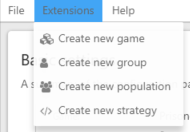
\includegraphics[width=0.4\linewidth]{img_manual/menubar_extensions.png}
\end{figure}

\subsection{Create new games}
When the \enquote{Create new game} entry in the \enquote{Extensions} menu is pressed, the game creation window opens (see Fig.\ref{fig:game_window}). Here, a new game can be created. To do so, a name, a description and the players payoffs must be entered in the corresponding text fields. For example, an entry of the form \enquote{\(1 / 2\)} in the botom left part of the payoff table means: \enquote{If player 1 doensn't but player 2 does cooperate, player 1 will receive the payoff \(1\) and player 2 will receive the payoff \(2\)}.

To reset all settings, press the  \inlinegraphics{img_manual/rotate_left_button.png} button.

To export the created game as a file, press the  \inlinegraphics{img_manual/export_button.png} button. To add the game to the local repository and close the window, press  \inlinegraphics{img_manual/check_button.png} (Further details and important information on exporting and saving see section \ref{sec:export_extensions}).

To load an existing game press the  \inlinegraphics{img_manual/import_button.png} button. The following dropdown menu will pop up:
\begin{figure}[h]
	\centering
	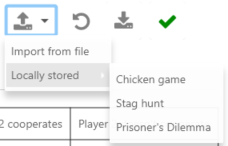
\includegraphics[width=0.4\linewidth]{img_manual/import_game.png}
\end{figure}\\
You can either import a game from a previously exported game file or open one of the locally stored games, i.e. the preconfigured games and the ones added to the repository by the user.

\begin{figure}
	\centering
	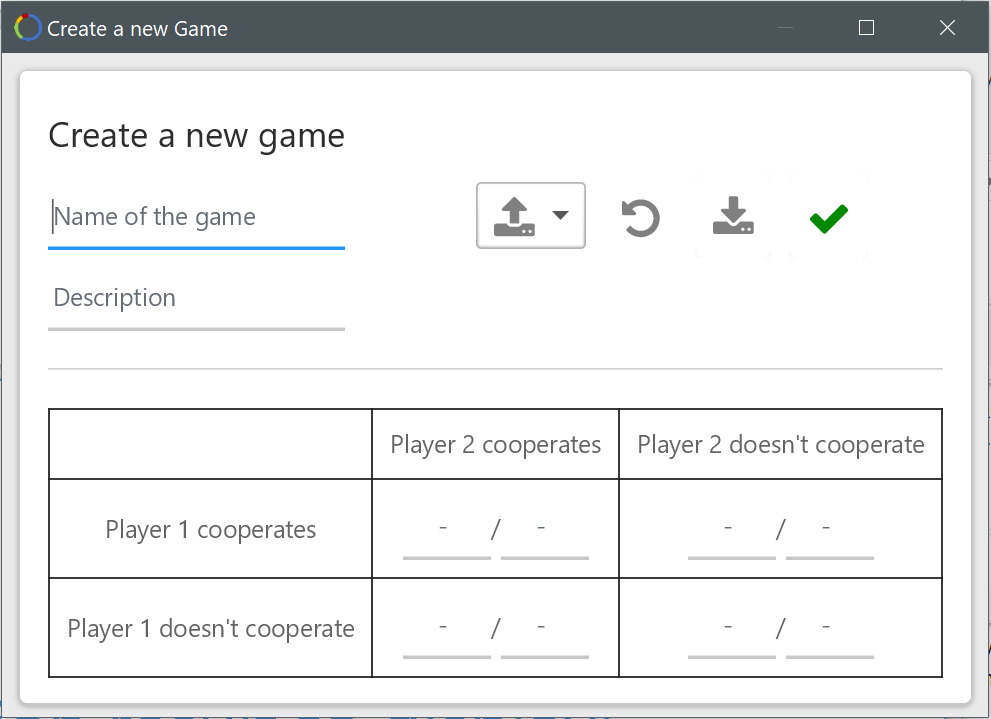
\includegraphics[width=0.8\linewidth]{img_manual/game_window.png}
	\caption{The game creation window.}
	\label{fig:game_window}
\end{figure}

\subsection{Create new strategies}

\subsection{Create new groups}
When the \enquote{Create new group} entry in the \enquote{Extensions} menu is pressed, the group creation window opens (see Fig.\ref{fig:group_window}). To create a new group, name and description must be entered in the corresponding text fields and at least one segment must be configured. Segments can be added by pressing the \enquote{Add segment} button and removed by pressing the \enquote{X} button at the head of the corresponding tab.

For each segment, a capital distribution must be chosen and parametrised; it will be used to initialise agents of that segment with capital at the beginning of simulations. Secondly, a set of strategies must be selected out of all locally stored strategies. Those include the preconfigured ones as well as strategies created by the user (if existent).

The multislider can be used to configure the relative sizes of the segments. For example, if \(100\) agents of the group in Fig.\ref{fig:group_window} were to be initialised, \(25\) of them would belong to segment 2, thus receiving an initial capital drawn out of a poisson distribution with mean \(15\) as well as \enquote{always cooperate} or \enquote{tit for tat} as initial strategy.

To reset all settings, press the  \inlinegraphics{img_manual/rotate_left_button.png} button.

To export the created group as a file, press the  \inlinegraphics{img_manual/export_button.png} button. To add the game to the local repository and close the window, press  \inlinegraphics{img_manual/check_button.png} (Further details and important information on exporting and saving see section \ref{sec:export_extensions}).

To load an existing group press the  \inlinegraphics{img_manual/import_button.png} button. You can either import a group from a previously exported game file or open one of the locally stored groups, i.e. the preconfigured groups and the ones added to the repository by the user.

\begin{figure}
	\centering
	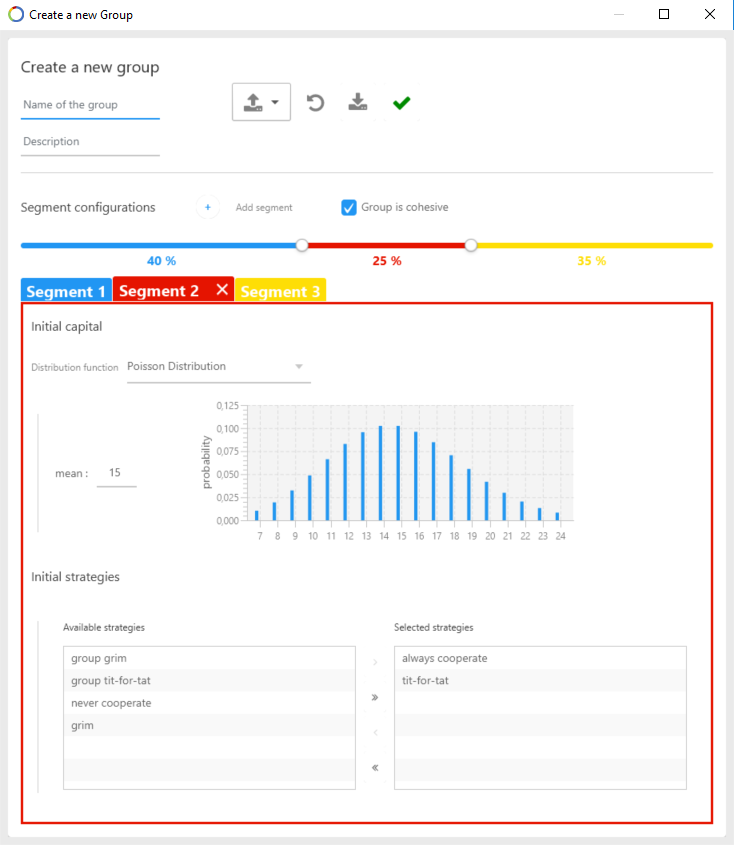
\includegraphics[width=0.8\linewidth]{img_manual/group_window.png}
	\caption{The group creation window.}
	\label{fig:group_window}
\end{figure}

\subsection{Create new populations}

\subsection{Important Information on Saving and Exporting Extensions}\label{sec:export_extensions}

\section{Advanced}

\subsection{Multiconfigurations}

\subsection{The Plugin-System}

\end{document}